\section{Clustering Method for Outlier Detection}
\label{sec:clusteroutlier}

It is important to detect outliers, to identify unusual behaviours shown by the employees. These outliers can also be used to highlight any possible imperfections in the data.

\subsection{Distance Measurement}
\label{sec:euclidean}

The definition of distance measurement between two data points is highly important in such a project, which uses spatial data. This project uses Euclidean distance and the distance $d(\bf{p},\bf{q})$ and is given in equation \ref{euclid}

\begin{equation}
\label{euclid}
d(\bf{p},\bf{q}) = \sqrt{(\bf{p}-\bf{q})\cdot(\bf{p}-\bf{q})}
\end{equation}



\subsection{Time of Day Comparison}
\label{sec:outliertimeday}

Data of interest is the comparison of the total distance travelled at different times of the day during the 14 day period. For this type of analysis the total distance travelled on weekends has been removed from the data set, since weekday travelling patterns often differ distinctly from weekend travelling patterns. The two times of day that are compared are 10.00 am and 4.00 pm. The first time has been selected in order to contain all distance travelled from home to work. The second is chosen to include all travel within lunch hour activities, but to exclude all travel to home. The total distance travelled in the morning in comparison to the afternoon for each vehicle on each day over the two week period is collated and shown in Figure \ref{fig:mornaft}. 

\begin{figure}[!ht]
\centering
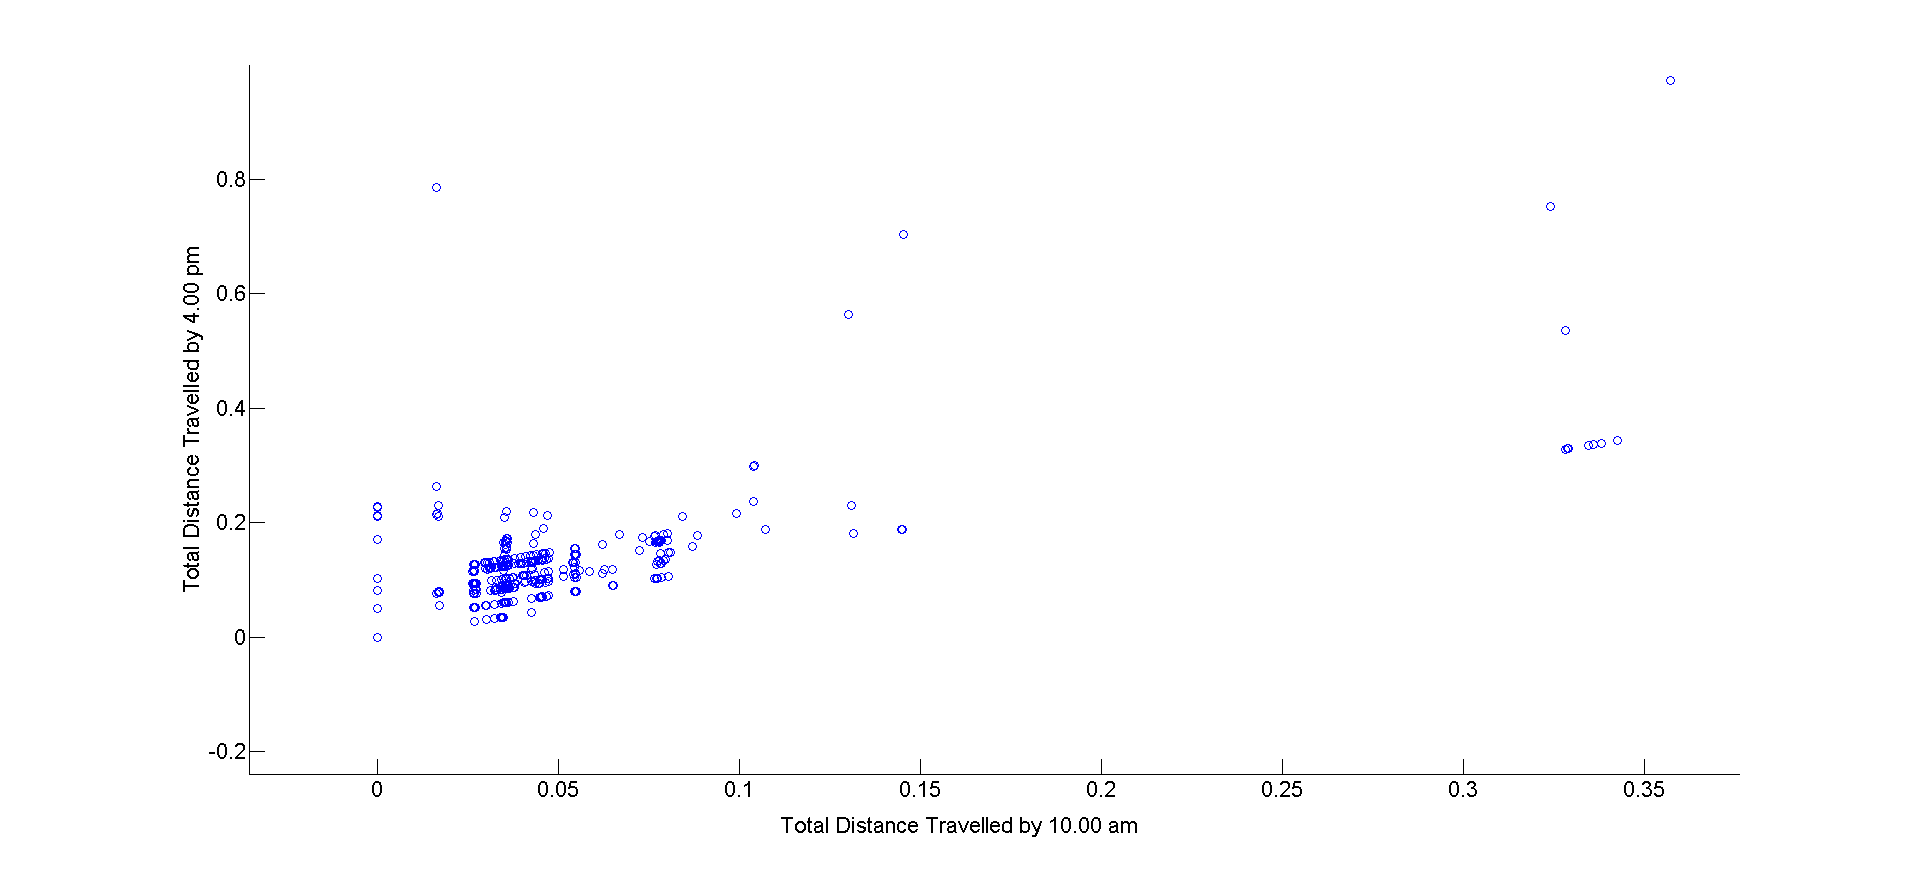
\includegraphics[width=1.1\textwidth]{Images/1stoutlier.png}
\caption{\label{fig:mornaft}Scattergraph showing total distance travelled at 10.00 am versus 4.00 pm for all vehicles for each weekday.}
\end{figure}

\noindent In Figure \ref{fig:mornaft} a high density area of data points can be seen with multiple outliers. To detect these outliers a method of cluster analysis can be used, and k-means clustering has been chosen for this set of data.



\subsection{K-means Clustering}
\label{sec:kmeans}

\noindent  K-means clustering is a centroid based classification system, and works by  creating number $k$ centroids, which are random points within the space.   Each of the $n$ observations into one of $k$ clusters; the cluster with the nearest mean in distance. The mean is then recalculated from these new clusters, and the algorithm repeats until the centroids no longer move location. A local optimum has been found. K-means clustering again relies on Euclidean distance. However a drawback of the k-means clustering set is the number of clusters within the data set must be determined beforehand. 



\subsection{Determining Number of Clusters}
\label{determinenocluster}


One approach to determine the appropriate number of clusters is to look at the within class variance $\sigma^2_{W}$ and between class variance $\sigma^2_{B}$, which are given in equations (\ref{OB}) and (\ref{OW}) . $N$ is the total number of data points, $K$ is the number of clusters and $C_{k}$  is the number of elements in cluster k. Lastly $\bar(x)$ is the mean of all data.
\begin{equation}
\label{OW}
\sigma^2_{W} = \frac{1}{N}\sum_{k = 1}^{K}\sum_{i = 1}^{C_{k}}[(x_{i} - \mu_{k})(x_{i} - \mu_{k})^T]
\end{equation}

\begin{equation}
\label{OB}
\sigma^2_{B} = \frac{1}{N}\sum_{k = 1}^{K} C_{k}[(\mu_{k}-\bar{x})(\mu_{k}-\bar{x})^T]
\end{equation}


\noindent It is desirable that a clustering algorithm produces results where each cluster is of a high density, and each cluster is far removed from any other cluster. In other words, the optimisation problem is to minimise $\sigma^2_{W}$ and to maximise $\sigma^2_W$. However the sum of within- and between- class variance is equal to the variance of the data, which is constant. Hence minimising $\sigma^2_{W}$ and maximizing $\sigma^2_W$ is the same optimisation problem, and the focus can be placed on $\sigma^2_{W}$ . The plot of the number of clusters versus $\sigma^2_{W}$ is shown in Figure \ref{fig:elbow}.\cite{cluster}



%will change this graph in the morning
\begin{figure}[!ht]
\centering
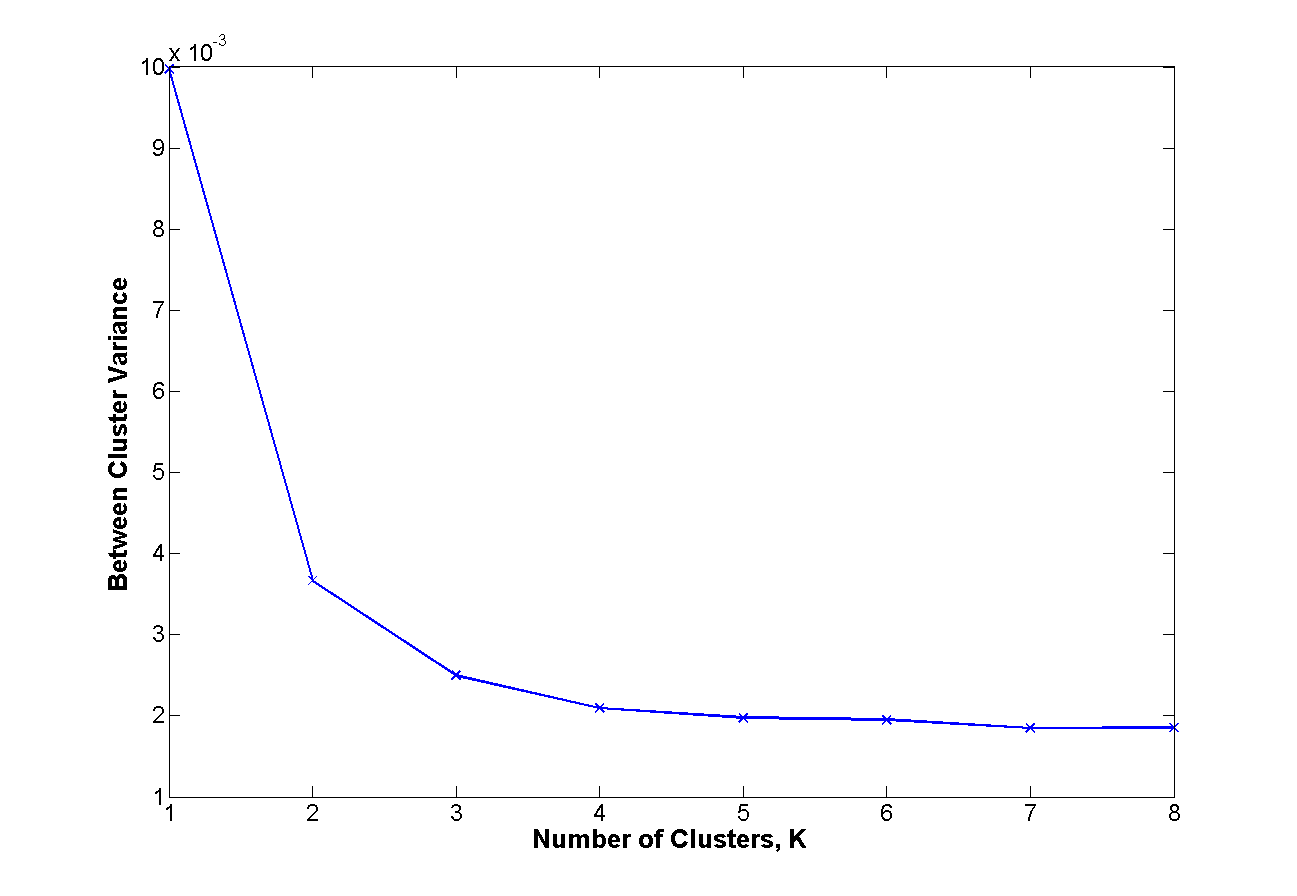
\includegraphics[width=1.0\textwidth]{Images/Sw2graph.png}
\caption{\label{fig:elbow} Graph showing the relationship between number of clusters and Between-class Variance  }
\end{figure}






% %will change this graph in the morning
% \begin{figure}[!ht]
% \centering
% 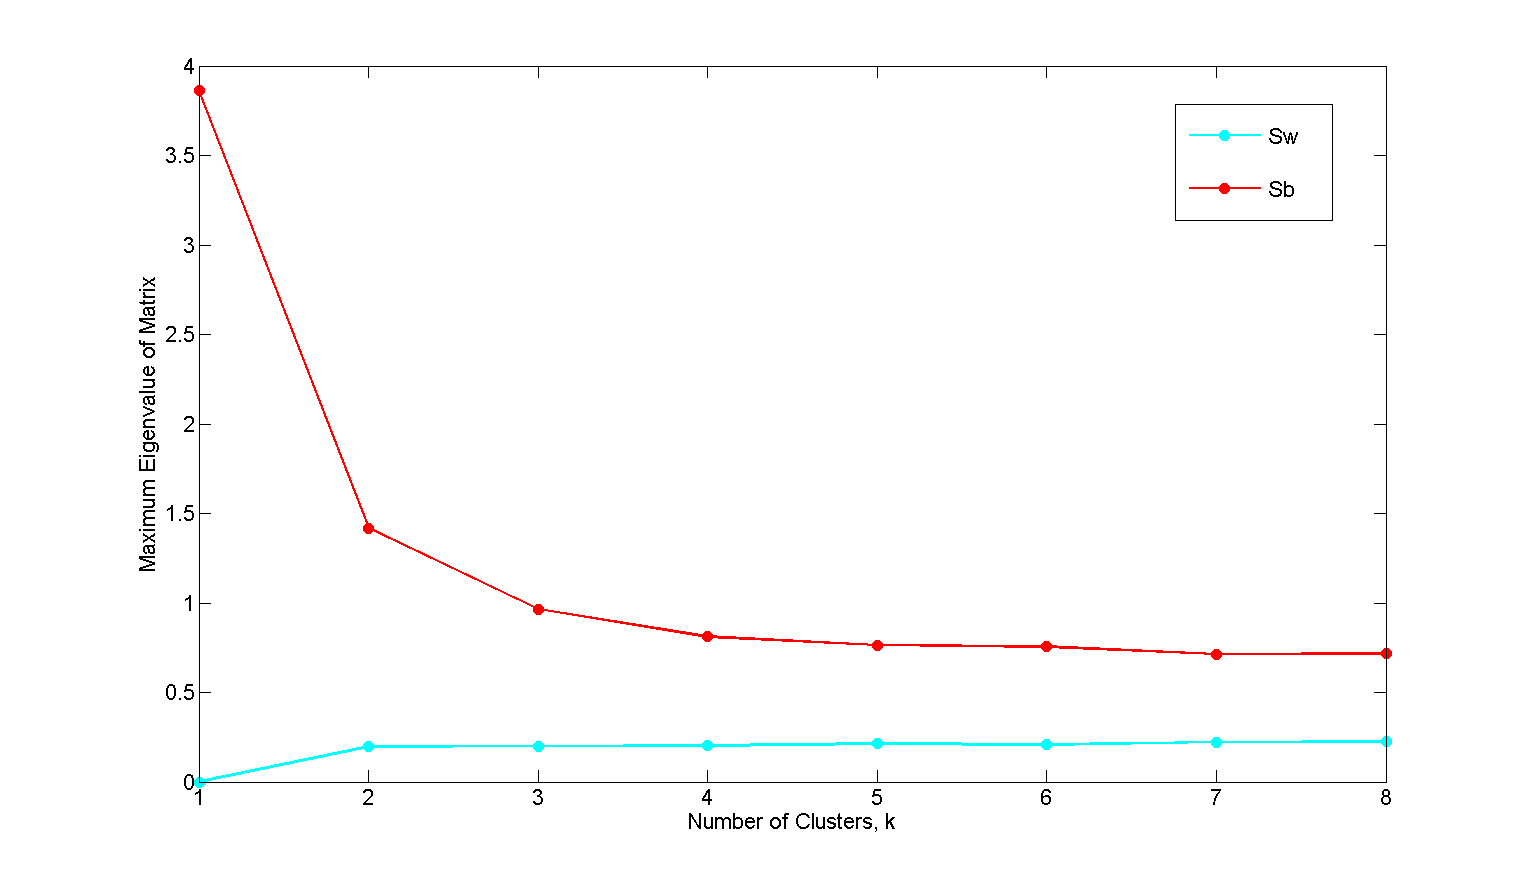
\includegraphics[width=0.8\textwidth]{Images/Swsbgraph.png}
% \caption{\label{fig:elbow} Number of Clusters against the maximum eigenvalue of the scatter matrix }
% \end{figure}



\noindent Figure \ref{fig:elbow} shows that $\sigma^2_{W}$ decreases as the number of clusters increases. This will continue until $K = N$, where each data point is defined as a cluster.\\

\noindent However, a trade off between model accuracy and complexity should be taken into account and so the elbow point should be studied. The elbow point for $\sigma^2_{W}$ is $K = 3$ and so this should be taken as the appropriate value for the model. The clustering algortithm with $k  =3$ is shown in Figure \ref{fig:4cluster}.



\begin{figure}[!ht]
\centering
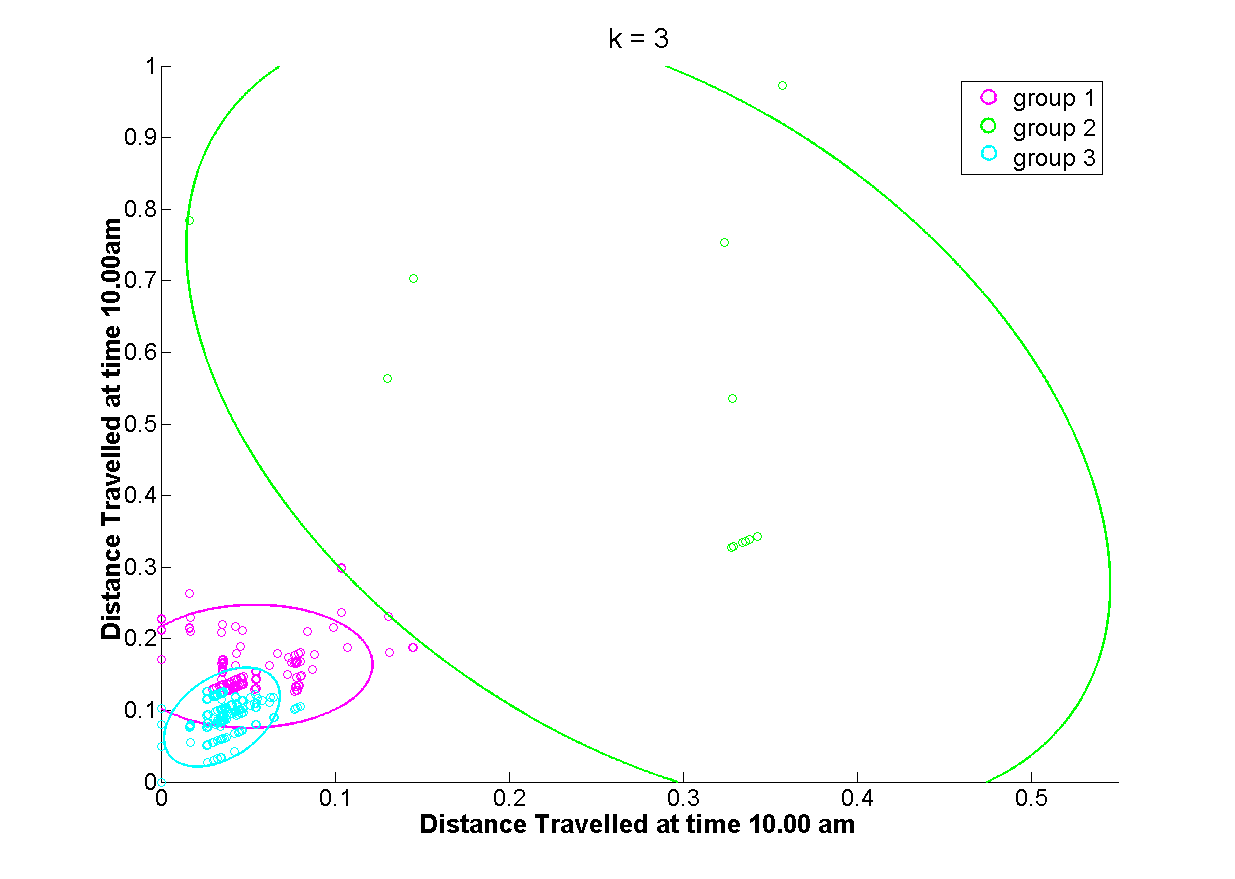
\includegraphics[width=0.7\textwidth]{Images/4cluster.png}
\caption{\label{fig:4cluster} Results of k-means clustering with k = 3. Ellipses contain 95\% of the data within the cluster.}
\end{figure}





\subsection{Outlier Identification}
\label{sec:outliers}
From the results of the k-means clustering the outliers can be identified. It can be seen that members in group 2 are outliers. This is because the two other groups have a visibally smaller within cluster variance , and group 2 is much bigger and removed. These values are summarised in Table \ref{table:outliers}. Further investigation will be carried out on Elsa Orilla, as she is consistently travelling a much further distance than any other individual, which can been seen in section 5.2.


\begin{table}[H]
\begin{center}
\begin{tabular}{|l|l|}
\hline  
Person & Day  \\ \hline \hline
Elsa Orilla     &   1,2,3,4,5,8,9,10,11,12   \\ \hline
Willem Vasco-Pais    &  5,11   \\ \hline
Valeria Morlun, Adan Morlun, Cecili Morluniau&    12   \\ \hline

\end {tabular}
\caption{\label{table:outliers}Outliers identified by K-means Clustering Method}
\end{center}
\end{table}

%\clearpage



